\subsection{Historique}

	Les premiers usages étaient pour les militaires.
	Les exemples les plus connus sont :
	\begin{itemize}
		\item[\textbullet] chiffrement par décalage, ou de Jules César,
		\item[\textbullet] chiffrement par substitution, on applique une fonction de permutation sur les lettres,
		\item[\textbullet] chiffrement par permutation : on divise le texte en groupes de lettres de même taille et à chaque groupe on applique une permutation entre les lettres.
	\end{itemize}
	
	La plupart des systèmes actuels peuvent se voir comme combinaisons de ces transformations élémentaires.
	
	\paragraph{Principe de Kerckhoff :} quasiment toutes les caractéristiques du système doivent être publiques, mais le chiffrement dépend juste d'un paramètre secret, la clé.
	
	Intérêt :
	\begin{itemize}
		\item[\textbullet] déploiement à grande échelle,
		\item[\textbullet] ne compromet pas toute la sécurité du système si une seule clé s'ébruite,
		\item[\textbullet] permet d'analyser la sécurité par des tiers.\\
	\end{itemize}
	
	Peut-on prouver qu'un système est sûr, mesurer sa sécurité ?
	Deux approches possibles :
	\begin{itemize}
		\item[\textbullet] sécurité informationnelle \textrightarrow\ théorie de l'information (Shannon).\\
			1948 : \textit{A mathematical theory of communications}\\
			1949 : \textit{Communication theory of secrecy systems}
		\item[\textbullet] sécurité computationnelle \textrightarrow\ théorie de la complexité.
	\end{itemize}


\subsection{Sécurité informationnelle}

	\begin{center}
	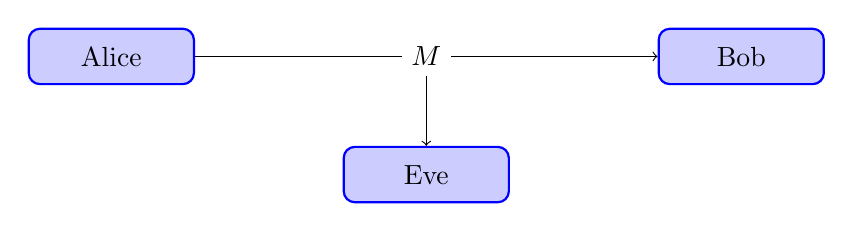
\begin{tikzpicture}
		\tikzstyle{block} = [rectangle, draw=blue, thick, fill=blue!20, text width=5.3em, text centered, rounded corners, minimum height=2em]
		\node [block] (A) at (0,0) {Alice};
		\node (X) at (4,0) {$M$};
		\node [block] (B) at (8,0) {Bob};
		\node [block] (E) at (4,-1.5) {Eve};
		\draw      (A) to (X);
		\draw [->] (X) to (B);
		\draw [->] (X) to (E);
	\end{tikzpicture}
	\end{center}
	
	Modèle : A veut envoyer un message clair $M \in \mathcal{M}$. $M$ est vu comme une variable aléatoire de loi donnée.
	
	\begin{defn}
		\textbf{Fonction de chiffrement} : $E \colon \mathcal{M} \times \mathcal{K} \to \mathcal{C}$ où $\mathcal{K}$ est l'espace des clés et $\mathcal{C}$ est l'espace des chiffrés.
	\end{defn}
	
	Au préalable Alice et Bob se sont mis d'accord sur une clé $K \in \mathcal{K}$.
	$K$ est également vue comme une v.a de loi donnée.\\
	
	Alice envoie à Bob le chiffré $C = E_K(M)$.
	Eve voit donc passer $C$.
	Quelle information peut-elle en déduire sur $M$ ?
	

\subsection{Les systèmes parfaits}
	
	\begin{defn}
		Dans un \textbf{système parfait au sens de Shannon}, la connaissance de $C$ n'apporte aucune info sur $M$.
	\end{defn}
	
	Deux variantes :
	\begin{itemize}
		\item[\textbullet] \textit{en moyenne} : $H(M \mid C) = H(M)$,
		\item[\textbullet] \textit{dans tous les cas} : égalité des lois, $\forall M, \forall C, p(M \mid C) = p(M)$.
	\end{itemize}
	
	\begin{ex}
		On a les données suivantes :
		$$\mathcal{M} = \{ \text{oui}, \text{non} \}, \quad p(\text{oui}) = \frac{3}{4}, p(\text{non}) = \frac{1}{4}, \quad
		\mathcal{K} = \{ K_1, K_2, K_3 \}, \quad p(K_1) = p(K_2) = p(K_3) = \frac{1}{3}, \quad
		\mathcal{C} = \{ x, y, z \}$$
		
		et le chiffrage donné par
		$\begin{array}{l|ll}
		    & \text{oui} & \text{non} \\
		K_1 & $x$        & $y$ \\
		K_2 & $y$        & $x$ \\
		K_3 & $z$        & $y$ \\
		\end{array}$.
		
		Eve voit $C$ et en déduit que Alice a envoyé $M$ avec probabilité $p(M \mid C)$.
		Par formule de Bayes il vient $p(\text{oui} \mid x) = \frac{ p(x \mid \text{oui}) p(\text{oui}) }{p(x)}$, avec $p(x) = p(x \mid \text{oui}) p(\text{oui}) + p(x \mid \text{non}) p(\text{non})$ et idem avec $y$ et $z$ ou $M = \text{oui}$.
		
		On trouve $p(x) = \frac{1}{3}$, $p(y) = \frac{5}{12}$ et $p(z) = \frac{1}{4}$.
		
		Supposons $C = x$.
		Alors $p(\text{oui} \mid x) = \frac{3}{4}$ et $p(\text{non} \mid x) = \frac{1}{4}$ donc Eve n'a rien appris de plus que ce qu'elle connaissait déjà.
		
		Supposons $C = y$.
		Alors $p(\text{oui} \mid y) = \frac{3}{5}$ et $p(\text{non} \mid y) = \frac{2}{5}$.
		L'incertitude est plus grande, en un sens Eve a appris quelque chose de nouveau par rapport à ce qu'elle estimait précedemment.
		
		Supposons $C = z$.
		Alors $p(\text{oui} \mid z) = 1$ et $p(\text{non} \mid z) = 0$.
		Donc le clair se déduit du chiffré.
		
		En conclusion ce système n'est pas parfait.
	\end{ex}
	
	\begin{ex}[Un système parfait : le one-time pad, ou masque jetable]
		On prend $\mathcal{M} = \{ 0, 1 \}^n$, $\mathcal{K} = \{ 0, 1 \}^n$ avec une distribution uniforme des clés et $\mathcal{C} = \{ 0, 1 \}^n$.
		On prend $E_K(M) := M \oplus K$.
		Alors $\forall M, \forall C, p(M \mid C) = p(M)$.
		Cette méthode est lourde : clé de même longueur que le message.
	\end{ex}
	
	\begin{thm}
		Dans un système parfait on a nécessairement $\card(\mathcal{K}) \geq \card(\mathcal{C})$.
	\end{thm}
	
	\begin{proof}
		Pour un $M$ donné on a
		$$\forall C, p(C \mid M) = \frac{p(C,M)}{p(M)} = \frac{p(C \mid M)}{p(M \mid C)} = p(C) > 0$$
		donc il existe une clé $K$ telle que $C = E_K(M)$, d'où le résultat.
	\end{proof}
	
	\begin{rem}
		On a toujours $\card(C) \geq \card(M)$ pour pouvoir opérer un décodage (fonction $E$ injective).
		Le cas le plus économique en sytème parfait est donc $\card(\mathcal{K}) = \card(\mathcal{C}) = \card(\mathcal{M})$ et alors $\forall M, \forall C, \exists ! K, C = E_K(M)$.
	\end{rem}
	
	On peut ensuite en déduire que la distribution de $K$ doit être uniforme \textrightarrow\ c'est le one-time pad.


\subsection{Distance d'unicité}

	Scénario : réutilisation d'une même clé pour chiffrer plusieurs messages.
	
	\begin{ex}[Chiffrement par substitution]
		On prend $\mathcal{M} = \mathcal{C} = \{ \mathsf{A},\mathsf{B},\mathsf{C},\ldots,\mathsf{Z} \}$ et $\mathcal{K}$ l'ensemble des permutations de $\mathcal{M}$.
		La réutilisation d'une clé permet d'étendre $E \colon \mathcal{M} \times \mathcal{K} \to \mathcal{C}$ en $E \colon \mathcal{M}^n \times \mathcal{K} \to \mathcal{C}^n$.
		
		Ce système s'attaque par analyse des fréquences dès lors qu'on sait que le clair est restreint à un certain sous-ensemble de $\mathcal{M}^n$, e.g texte en français qui n'est pas une suite de lettres “très aléatoire”.
	\end{ex}
	
	Question : à partir de quelle longueur de chiffré peut-on retrouver la permutation clé ?
	
	Prenons un alphabet $\mathcal{A}$.
	Alors $\mathcal{M} = \mathcal{A}^n$ avec une certaine redondance (non uniformité dans $\mathcal{A}$).
	
	\begin{defn}
		\textbf{Entropie du langage} : $h = \lim_{n \to \infty} \frac{1}{n} H(M)$.
	\end{defn}
	
	\begin{defn}
		\textbf{Redondance du langage} : $r = 1 - \frac{h}{\log_2(\card(\mathcal{A}))}$.
	\end{defn}
	
	Intuitivement un texte de $n$ symboles dans le langage peut se compresser en $nh$ bits ($n \to \infty$).
	
	En longueur $n$, parmi les $\card(A)^n$ suites de $n$ symboles possibles, il y en a $\simeq 2^{nh}$ qui sont dans le langage.
	Les chiffrés doivent sembler aléatoires, on peut espérer en avoir $\card(A)^n$.
	
	À chaque chiffré correspond $\displaystyle \frac{2^{nh + \log_2(\# \mathcal{K})}}{(\# \mathcal{A})^n}$ couples $(M,K)$ possibles.
	
	Une recherche exhaustive donne un déchiffrement unique dès lors que $\frac{2^{nh + \log_2(\# \mathcal{K})}}{(\# \mathcal{A})^n} \leq 1$, où $\frac{2^{nh + \log_2(\# \mathcal{K})}}{(\# \mathcal{A})^n} = 2^{n(h - \log_2 \# \mathcal{A}) + \log_2 \# \mathcal{K}} = 2^{-rn \log_2 \# \mathcal{A} + \log_2 \# \mathcal{K}}$.
	
	\begin{defn}
		\textbf{Distance critique} : $n = \frac{\log_2 \# \mathcal{K}}{r \log_2 \# \mathcal{A}}$.
	\end{defn}
	
	\begin{ex}
		Pour une substitution simple, en français, $\# \mathcal{K} = 26!$, donc $\log_2 \# \mathcal{K} \simeq 88$, $r \in \inff{0{,}75}{0{,}8}$ et $\# \mathcal{A} = 26$ donc $\log_2 \# \mathcal{A} \simeq 4{,}7$.
		Alors $n \simeq 25$.
		En pratique, à la main, on peut casser le chiffrement pour $n$ jusqu'à 200 ou 250.
	\end{ex}
	
	Autre exemple avec sécurité informationnelle : partage de secret à seuil.
	
	\begin{ex}[Le système de Shamir]
		Un “distributeur” dispose d'un secret $S \in \F_q$ et veut donner une part de ce secret à $n$ participants de sorte que :
		\begin{itemize}
			\item[\textbullet] $t$ participants qui se concertent peuvent reconstruire le secret avec leurs parts,
			\item[\textbullet] $t - 1$ participants n'ont aucune info sur $S$.
		\end{itemize}
		
		On supposera $q > n$.
		Le distributeur choisit $t - 1$ éléments $a_1,\ldots,a_{t-1} \in \F_q$ uniformément indépendants.
		Il prend le polynôme $P(X) = S = a_1 X + a_2 X^2 + \ldots + a_{t - 1} X^{t - 1}$.
		
		Étant choisis $x_1,\ldots,x_n \in \F_q^\times$ distincts, on calcule $y_i = P(x_i)$.
		Au participant n°$i$ est envoyé le couple $(x_i,y_i)$.
		L'assignation des $x_i$ peut être publique, la part de secret est contenue dans $y_i$.
		
		Cela vérifie bien les propriétés voulues :
		\begin{itemize}
			\item[\textbullet] Si $t$ participants se concertent $P$ est déterminé de façon unique par interpolation de Lagrange : $P(X) = \sum_{i = 1}^t y_i \prod_{j \neq i} \frac{X - x_i}{x_i - x_j}$ et alors $S = P(0)$.
			\item[\textbullet] Si $t - 1$ participants se concertent ils ne peuvent en déduire aucune information car toutes les valeurs de $S$ sont compatibles par interpolation de Lagrange.
		\end{itemize}
	\end{ex}


\subsection{Sécurité computationnelle}

	En cryptographie symétrique, A et B possèdent une clé secrète commune.
	En cryptographie asymétrique on veut communiquer de façon sécurisée sans avoir eu la possibilité au préalable de se mettre d'accord sur un secret commun.
	
	Historique : 1974, Merkle, projet de fin d'études \textit{Énigmes}.
	
	Bob prépare un grand nombre $N$ de messages clairs qui disent « la clé n°$i$ est $k_i$ ».
	Il les chiffre de façon pas très sûre, cassable en temps $T$.
	Il publie ces chiffres (dans le désordre).
	
	Alice choisit une devinette, elle la résout et apprend un couple $(i,k_i)$.
	Elle dit à Bob « je connais la clé n°$i$ ».
	Eve ne sait pas quelle devinette correspond à la clé $i$, elle doit les résoudre toutes \textrightarrow\ en moyenne temps $\frac{N}{2} T$.
	
	\begin{ex}[\textbf{Diffie-Hellman} (1976)]
		Système d'échange de clé (key agreement).
		
		\begin{table}\centering
		\begin{tabular}{aca}
			Alice & \textit{Public} & Bob \\
			\hline
			 & $\F_q$ & \\
			 & $\alpha \in \F_q^\times$ & \\
			$r \in \Z$ aléatoire & & $s \in \Z$ aléatoire \\
			$\beta = \alpha^r$ & $\overset{\beta}{\longrightarrow} $ & \\
			 & $\overset{\gamma}{\longleftarrow}$ & $\gamma = \alpha^s$ \\
			$\gamma^r = \alpha^{rs}$ & & $\beta^s = \alpha^{rs}$
		\end{tabular}
		\end{table}
		
		À la fin $\alpha^{rs}$ est leur secret commun.
		Eve voit passer $q,\alpha,\beta,\gamma$.
		Elle doit en déduire un certain $\delta$ tel que $\exists r,s, \delta = \alpha^{rs}, \beta = \alpha^r, \gamma^s$.
		C'est le \textit{problème de Diffie-Hellman}.
		Cela ressemble (mais n'est pas équivalent) au problème du log discret : connaissant $q,\alpha,\beta$, trouver $r$ tel que $\beta = \alpha^r$.
	\end{ex}
	
	\begin{ex}[\textbf{RSA}, 1978]
		Méthode de chiffrement et de signature.
		
		Bob choisit $p$ et $q$ premiers secrets.
		Il calcule $N = pq$, alors $\varphi(N) = (p - 1)(q - 1)$.
		Il choisit $e \in \N$ premier à $\varphi(N)$ et $d$ son inverse, i.e $ed = 1 \mod{\varphi(N)}$.
		
		La clé publique de Bob est $(N,e)$, où $N$ est appelé \textit{module RSA} et $e$ est l'\textit{exposant de chiffrement}.
		L'entier $d$ sera appelé \textit{exposant de déchiffrement} et constitue la clé secrète.
		
		Alice veut envoyer un message clair à Bob encodé comme un élément $m \in (\Z / N\Z)^\times$.
		Elle calcule $c = m^e$, le chiffré, et l'envoie à Bob.
		Bob déchiffre $c^d = m^{ed} = m$.
		
		Eve peut vouloir :
		\begin{enumerate}[1 -]
			\item retrouver le secret primitif de Bob, i.e $p$ et $q$, ensuite elle trouve $\varphi(N)$ puis $d = e^{-1}$ par Euclide,
			\item retrouver juste $d$ à partir de $(N,e)$,
			\item être capable de retrouver un $m$ correspondant à un $c$,
			\item retrouver un bit d'information sur $m$ à partir de $c$ où $m$ est vu comme un entier dans $\iniff{1}{N - 1}$.
		\end{enumerate}
		
		Remarque : en théorie de la complexité on appelle “faciles” les problèmes résolubles en temps polynomial en la taille des entrées.
		On appelle difficile les problèmes résolubles en tant exponentiel \textrightarrow\ sous classe NP.
		
		En crypto on veut typiquement que le déchiffrement soit NP : facile si on connaît la clé et difficile si on ne la connaît pas.
		
		Dans le cas de RSA :
		\begin{enumerate}[1 \textrightarrow\ ]
			\item problème de factorisation donné $N$, trouver ses facteurs premiers $p$ et $q$.
				Le problème est réputé NP, mais ni P ni NP-complet.
			\item on peut montrer que ça équivaut à 1.
			\item extraction de racine $e$\up{ième} dans $\Z / N\Z$, $m = \sqrt[e]{c} \mod{N}$.
				Si $e = 2$ on a vu que c'était équivalent à la factorisation de $N$.
				Mais lorsque $e$ est impair (souvent $e = 3$), cela pourrait être plus facile quee la factorisation mais estimé non polynomial.
			\item équivalent à 3.
				Plus précisément on a une réduction polynomiale de l'un à l'autre.
				Soit $A$ une “boîte noire” qui nous dit si $m < \frac{N}{2}$ ou non à partir du chiffré $c$.
				Or on a $2^e c = (2m)^e$ le chiffré correspondant au clair $2m \mod{N}$.
				Si $m < \frac{N}{2}$, $2m \mod{N} = 2m$ pair et si $m > \frac{N}{2}, 2m \mod{N} = 2m - N$ impair.
				Ensuite, par dichotomie, en $\log_2(N)$ appels à la boîte $A$ on a complètement localisé $m$.
		\end{enumerate}
	\end{ex}
	
	\begin{ex}
		Public : $\F_q$ et $\alpha \in \F_q^\times$.
		Clé publique de Bob : $\beta \in \F_q^\times$.
		Clé secrète : $r \in \Z$ tel que $\beta = \alpha^r$.
		
		Alice veut envoyer le message en clair $m \in \F_q^\times$.
		Elle choisit $s \in \Z$ aléatoire et calcule $c_1 = \alpha^s$ et $c_2 = \beta^s m$.
		Elle envoie $(c_1,c_2)$ à Bob qui déchiffre par $c_2 c_1^{-r} = \beta^s m \alpha^{-rs} = m$.\\
		
		\noindent Eve peut vouloir :
		\begin{enumerate}[1.]
			\item retrouver la clé secrète à partir de la clé publique \textrightarrow\ problème du logarithme discret,
			\item retrouver $m$ à partir de $(c_1,c_2)$ où sont connus $F_q, \alpha, \beta = \alpha^r, c_1 = \alpha^s, c_2 = m \alpha^{rs}$.
				Alors retrouver $m$ revient à retrouver $\alpha^{rs}$.
				C'est le problème de DH.
		\end{enumerate}
		
		DH et El Gamal utilisent la structure de groupe de $\F_q$.
		La sécurité repose essentiellement sur la difficulté du log discret dans ce groupe.
		De même que la factorisation on ne sait pas le résoudre en temps polynomial, mais on sait faire mieux que exponentiel.
		
		Formule générale : $L_{\varepsilon,c}(t) = \exp \left( c \cdot t^\varepsilon \log(t)^{1 - \varepsilon} \right)$.
		Si $\varepsilon = 0$ on est dans le cas polynomial : $L_{\varepsilon,c}(t) = t^c$.
		Si $\varepsilon = 1$ on est dans le cas exponentiel : $L_{\varepsilon,c}(t) = e^{ct}$.
		
		On sait résoudre les problèmes de factorisation et de log discret en $\varepsilon = \frac{1}{3}$.
		En pratique, avec les puissances de calcul actuelles, cela veut dire que l'on doit prendre des clés de taille environ 2000 bits.
	\end{ex}